\documentclass[10pt]{article}
\usepackage{amsmath}
\usepackage{mathtools}
\DeclarePairedDelimiter{\abs}{\lvert}{\rvert}
\usepackage[hidelinks]{hyperref}
\usepackage{amssymb}
\usepackage{tikz}
\usepackage{caption}
\usepackage{graphicx}
\usepackage[T1]{fontenc}
\graphicspath{{.}}
\usepackage{listings}
\usepackage{verbatim}
\usepackage{floatrow}
\usepackage{bigints}
\lstset{
language=[LaTeX]TeX,
backgroundcolor=\color{gray!25},
basicstyle=\ttfamily,
columns=flexible,
breaklines=true
}
\captionsetup{labelsep=colon,justification=centering,singlelinecheck=off}
\reversemarginpar
\usepackage[paper=a4paper,
            %includefoot, % Uncomment to put page number above margin
            marginparwidth=10mm,      % Length of section titles
            marginparsep=0.8mm,       % Space between titles and text
            margin=11mm,              % 25mm margins
            includemp]{geometry}

\begin{document}
\section*{}
\begin{flushleft}
Name: Krishna Chaitanya Sripada\\
\end{flushleft}
\section*{Ans 13}
\begin{flushleft}
\begin{lstlisting}
function adjMat= adjMatrix(p,q,n)
I = eye(n);
ix = randperm (n);
T = I(ix,:);
n2 = n/2;
P = random('bino', 1, p, n2, n2); 
dP2 = random('bino', 1, p, n2, 1); 
Q = random('bino', 1, q, n2, n2); 
U = triu(P, 1);
L = tril(P,-1);
dP = diag(P);
A0 = U + U' + diag(dP);
A1 = Q;
A2 = Q';
A3 = L + L' + diag(dP2);
A =[A0 A1;A2 A3];
adjMat = T*A*T.';
end \end{lstlisting}
\end{flushleft}
\section*{Ans 14}
\begin{flushleft} 
\begin{lstlisting}
function [community1, community2] = partition(p,q,n)
adjMat = adjMatrix(p,q,n);
[V,D] = eig(adjMat);
secondDomEigenVector = V(:,n-1);
community1=[];
community2=[];
for i=1:n
    if secondDomEigenVector(i)>0
        community1 = [community1 i];
    else
        community2 = [community2 i];
    end
end
\end{lstlisting}
\end{flushleft}
\section*{Ans 15}
\begin{flushleft}
The value of overlap when $\widetilde{\omega} = \omega$ is 1. The following is the program for that: \\
\begin{lstlisting}
function [overlap] = answer_15(p,q,n,T)
adjMatrixT = adjMatrix(1,0,n,T);
[V,D] = eig(adjMatrixT);
[X,Y] = sort(max(abs(D)), 'descend');
secondDEVT = V(:,Y(2));
for i=1:numel(secondDEVT)
    element = abs(secondDEVT(i));
    if element+1 ~=1
        wT(i) = 1;
    else
        wT(i) = -1;
    end
end

adjMatrixR = adjMatrix(p,q,n,T);
[V,D] = eig(adjMatrixR);
[X,Y] = sort(max(abs(D)), 'descend');
secondDEVR = V(:,Y(2));
for i=1:numel(secondDEVR)
    element = secondDEVR(i);
    if element>0
        wR(i) = 1;
    else
        wR(i) = -1;
    end
end
rawoverlap = max(sum(wT==wR), sum(-wT==wR));
overlap = (2*(rawoverlap)/n) - 1;
end
\end{lstlisting}
To prove that a random guess for the detection of the communities returns overlap = 0, pass p = 0.5 and q=0.5 to the above method as parameters. In other cases where p$\neq$q, we see that overlap $\geq$0. 
\end{flushleft}
\section*{Ans 16}
\begin{flushleft}
\begin{lstlisting}
function answer_16()
n = 300;
score = [];
for alpha=5:50
    for beta=1:50
        p = (alpha * log(n))/n;
        q = (beta * log(n))/n;
        meanOverlap = 0;
        if p>=q
           for i=1:20
               I = eye(n);
               ix = randperm (n);
               T = I(ix,:);
               overlp = answer_15(p,q,n,T);
               meanOverlap = meanOverlap + overlp;
           end
           score(alpha,beta) =  meanOverlap/20;
        end 
    end
end
imagesc(score);
colorbar;
colormap(gray);
hold on;
for beta=1:50
    p = [1 -(0.3506 +(2*beta)) -(0.3506*beta)+(beta*beta)];
    r = roots(p);
    X(b) = r(1);
end
plot(1:b,X,'r','LineWidth',3);
\end{lstlisting}
\begin{figure}[!htb]
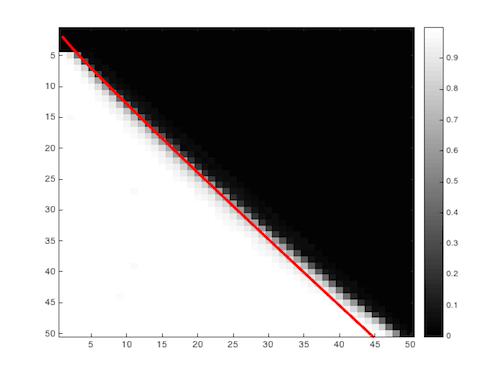
\includegraphics{16.png}
\caption{Probability of successfully detecting the partitions using the algorithm Partition for a dense network. x-axis corresponds to $\beta$ and y-axis corresponds to $\alpha$.}
\end{figure}
\end{flushleft}
\vspace{20em}
\section*{Ans 17}
\begin{flushleft}
\begin{lstlisting}
function answer_17()
n = 300;
score = [];
for a=5:70
    for b=1:50
        p = a/n;
        q = b/n;
        meanOverlap = 0;
        if p>=q
           for i=1:20
               I = eye(n);
               ix = randperm (n);
               T = I(ix,:);
               overlp = answer_15(p,q,n,T);
               meanOverlap = meanOverlap + overlp;
           end
           score(a,b) =  meanOverlap/20;
        end
    end
end
imagesc(score);
colorbar;
colormap(gray);
hold on;
for b=1:50
    p = [1 -((2*b)+1) +((b*b)-b)];
    r = roots(p);
    X(b) = r(1);
end
plot(1:b,X,'r','LineWidth',3)
\end{lstlisting}
\begin{figure}[!htb]
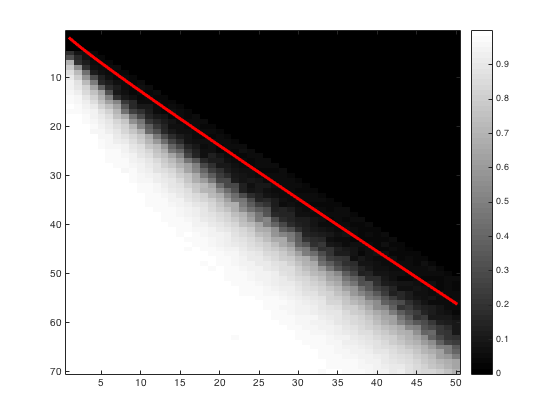
\includegraphics{17.png}
\caption{Probability of successfully detecting the partitions using the algorithm Partition for a sparse network. x-axis corresponds to $b$ and y-axis corresponds to $a$.}
\end{figure}
\end{flushleft}
\section*{Ans 18}
\begin{flushleft}
\begin{lstlisting}
function [wR] = answer_18(filename)
X = load(filename);
[V,D] = eig(X.A);
[X,Y] = sort(max(abs(D)), 'descend');
secondDEVR = V(:,Y(2));
for i=1:numel(secondDEVR)
    element = secondDEVR(i);
    if element>0
        wR(i) = 1;
    else
        wR(i) = -1;
    end
end
end\end{lstlisting}
The result is recovered partition returned is below:\\
\begin{lstlisting}
Columns 1 through 18

-1    -1    -1    -1    -1    -1    -1    -1     1     1    -1    -1    -1    -1     1     1    -1    -1

Columns 19 through 34

1     -1     1    -1     1     1     1     1     1     1     1     1     1     1     1     1
\end{lstlisting}
\end{flushleft}
\section*{Ans 19}
\begin{flushleft}
\begin{lstlisting}
function [ overlp ] = answer_19(wT, wR, n)
rawoverlap = max(sum(wT==wR), sum(-wT==wR));
overlp = (2*(rawoverlap)/n) - 1;
end
wT = [1 1 1 1 1 1 1 1 -1 -1 1 1 1 1 -1 -1 1 1 -1 1 -1 1 -1 -1 -1 -1 -1 -1 -1 -1 -1 -1 -1 -1];
\end{lstlisting}
The overlp value is 1 which means 100\% overlap.
\end{flushleft}
\end{document}